\documentclass{beamer}
\usepackage[utf8]{inputenc}
\usepackage[spanish]{babel}
\usepackage{graphicx}
\usepackage{hyperref}
\usetheme{Madrid}
\usepackage{fontawesome5}
\usepackage{graphicx}
\usepackage{pgfplots}
\usepackage{tabularx}
\usepackage{booktabs}  % para líneas horizontales más elegantes
\usepackage[table]{xcolor}  % opcional: para sombreado o color si lo deseas
\pgfplotsset{compat=1.17}

\title[Co-localización Ciencia y Tecnología]{The Organization of Corporate Science and Technology:\\ Out of Sight, Out of Mind?}
\subtitle{Grabowska (2021)}
\author{Bruno \textbf{CHAIHUAQUE}}
% \institute{Consorcio de Universidades}
\date{Doctorado en Gestión Estratégica}
\begin{document}
	
	\begin{frame}
		\centering
		\titlepage
		\vspace{1cm}
		
\includegraphics[width=0.9\textwidth]{./figs/Logos.pdf}
	\end{frame}
	
	% Slide: Objetivo
	\begin{frame}{Problema de investigación}
		\small
		\textit{Aunque las empresas biofarmacéuticas invierten significativamente en investigación científica, solo una fracción de estos descubrimientos se traduce en innovaciones tecnológicas (Gittelman \& Kogut, 2003).}
		
		\vspace{1em}
		\textbf{Tabla 1.} \textit{Principales economías por inversión en I+D}
		
		\vspace{0.5em}
		\renewcommand{\arraystretch}{1.1}
		\tiny
		\begin{tabularx}{\textwidth}{@{}l r X@{}}
			\toprule
			\textbf{Economía} & \textbf{Inversión media (M€)} & \textbf{Tres primeras empresas (y sector)} \\
			\midrule
			Estados Unidos & 31\,350 & 
			1. Alphabet (Software y servicios informáticos) \newline
			2. Meta (Software y servicios informáticos) \newline
			3. Microsoft (Software y servicios informáticos) \\
			\addlinespace
			
			China & 12\,282 & 
			1. Huawei Investment \& Holding (Aparatos y equipamientos tecnológicos) \newline
			2. Tencent (Software y servicios informáticos) \newline
			3. Alibaba Group Holding (Software y servicios informáticos) \\
			\addlinespace
			
			Alemania & 11\,633 & 
			1. Volkswagen (Automóviles y componentes) \newline
			2. Mercedes-Benz (Automóviles y componentes) \newline
			3. Robert Bosch (Automóviles y componentes) \\
			\addlinespace
			
			Suiza & 8\,241 & 
			1. Roche (Productos farmacéuticos y de biotecnología) \newline
			2. Novartis (Productos farmacéuticos y de biotecnología) \newline
			3. Nestlé (Producción de alimentos) \\
			\bottomrule
		\end{tabularx}
		
		\vspace{0.7em}
		\centering
		%\scriptsize \textit{Inversión en I+D de las principales economías}
	\end{frame}
	
	\begin{frame}{Objetivo del Estudio}
		\begin{itemize}
			\item Analizar cómo la \textbf{co-localización geográfica} de actividades científicas y tecnológicas en empresas biofarmacéuticas influye en la capacidad de explotar ciencia interna.
			\item Estudiar esta relación en el contexto de grandes empresas multinacionales con unidades dispersas.
		\end{itemize}
	\end{frame}
	
	% Slide: Marco Teórico
	\begin{frame}{Marco Teórico}
		\begin{itemize}
			\item La ciencia impulsa la innovación, pero su explotación es compleja.
			\item El conocimiento científico suele ser \textbf{tácito y contextual}.
			\item La proximidad facilita:
			\begin{itemize}
				\item Transferencia de conocimiento.
				\item Confianza y comunicación.
				\item Gestión conjunta de I+D.
			\end{itemize}
		\end{itemize}
	\end{frame}
	\begin{frame}{Modelo SECI}
		\centering
		\begin{minipage}{0.85\textwidth}
			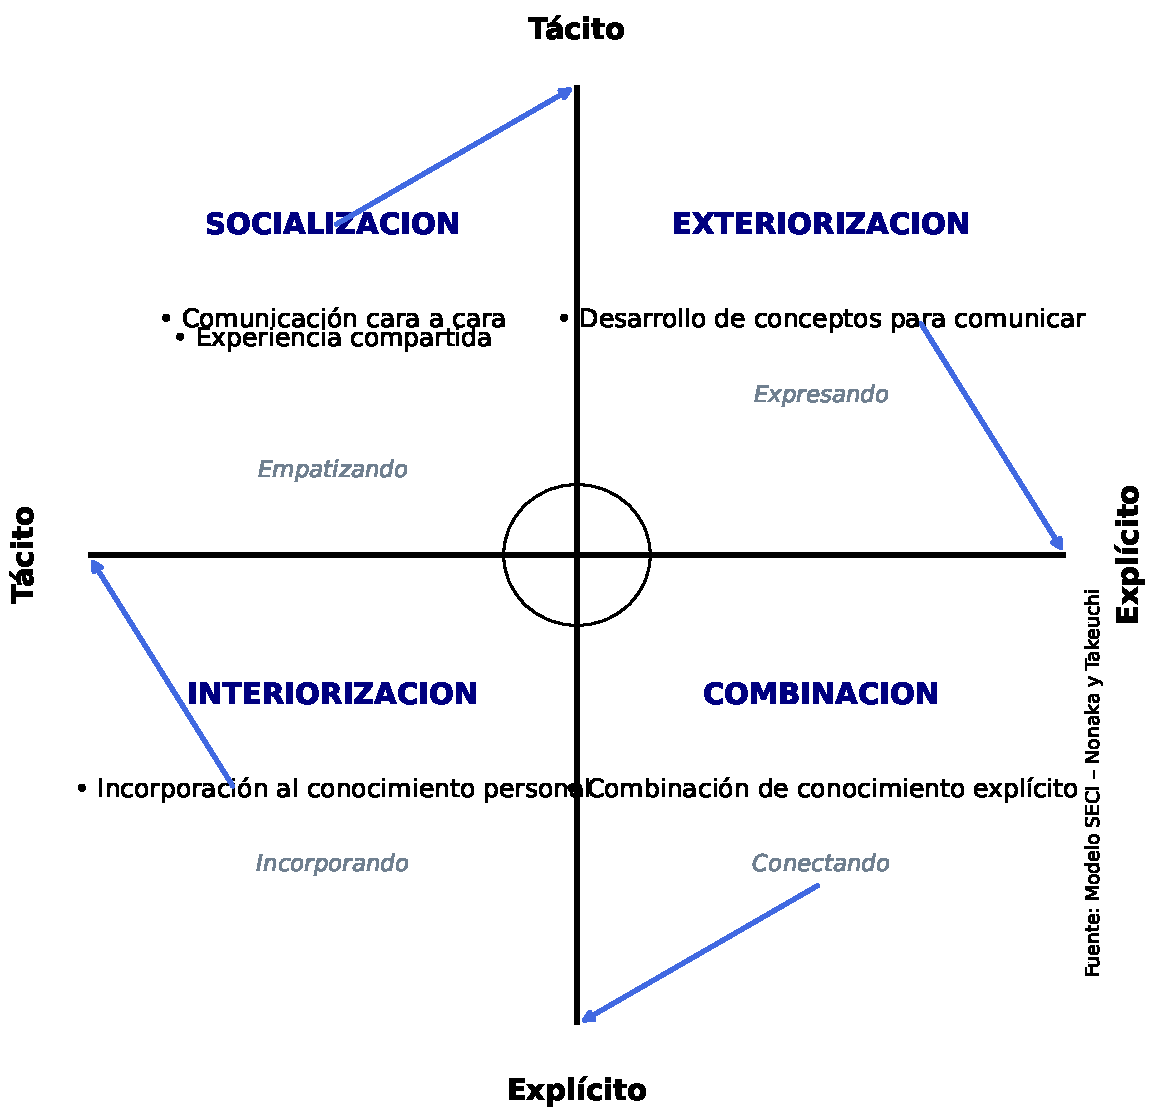
\includegraphics[width=0.8\textwidth]{./figs/Nonaka.pdf}
		\end{minipage}%
		\begin{minipage}{0.05\textwidth}
			\centering
			\rotatebox{-90}{\scriptsize Fuente: Nonaka \& Takeuchi (1995)}
		\end{minipage}
	\end{frame}
	
	% Slide: Hipótesis
	\begin{frame}{Hipótesis Principal}
		\begin{block}{H1}
			La co-localización de actividades científicas y tecnológicas está positivamente asociada con la explotación de ciencia interna en el desarrollo tecnológico.
		\end{block}
	\end{frame}
	
	% Slide: Metodología
	\begin{frame}{Metodología}
		\begin{itemize}
			\item Muestra: 227 empresas biofarmacéuticas (EE.UU., Europa, Japón).
			\item Periodo: 2000–2015.
			\item Datos:
			\begin{itemize}
				\item Publicaciones científicas (Web of Science).
				\item Patentes (PATSTAT).
			\end{itemize}
			\item Indicadores:
			\begin{itemize}
				\item \textbf{Co-localización}: coincidencia geográfica de autores e inventores.
				\item \textbf{Explotación científica}: citaciones internas de artículos en patentes.
			\end{itemize}
		\end{itemize}
	\end{frame}
	
	% Slide: Resultados
	\begin{frame}{Co-localización vs Explotación (U-shape)}
		\centering
		\begin{tikzpicture}
			\begin{axis}[
				width=9cm,
				height=5.5cm,
				xlabel={Índice de co-localización},
				ylabel={Explotación de ciencia},
				xmin=0, xmax=1,
				ymin=0.5, ymax=1.1,
				samples=100,
				domain=0:1,
				grid=both,
				axis lines=left,
				tick label style={font=\footnotesize},
				label style={font=\footnotesize},
				title style={font=\footnotesize},
				legend style={at={(0.5,-0.35)}, anchor=north, font=\scriptsize},
				title={Relación no lineal entre co-localización y explotación},
				]
				\addplot[blue, thick] {-10*(x - 0.65)^2 + 1};
				\addlegendentry{Explotación de ciencia propia}
				
				\addplot[red, dashed] coordinates {(0.65,0.5) (0.65,1.1)};
				\addlegendentry{Co-localización óptima (0.65)}
			\end{axis}
		\end{tikzpicture}
	\end{frame}
	\begin{frame}{Resultados Principales}
		\begin{itemize}
			\item Relación positiva: +8\% de explotación por 1 DE en co-localización.
			\item Relación curvilínea (U invertida): niveles altos reducen beneficios.
		\end{itemize}
		
	%	\pause
		\textbf{Posibles causas}:
		\begin{itemize}
			\item Competencia interna por recursos.
			\item Menor novedad científica si se orienta solo a fines tecnológicos inmediatos.
		\end{itemize}
	\end{frame}
	
	% Slide: Conclusiones
	\begin{frame}{Conclusiones}
		\begin{itemize}
			\item La estructura geográfica de I+D importa para la innovación.
			\item La co-localización:
			\begin{itemize}
				\item Favorece la transferencia de conocimiento.
				\item Pero puede limitar la creatividad si es excesiva.
			\end{itemize}
			\item Aporte: evidencia empírica sobre un mecanismo poco explorado en la organización de la I+D.
		\end{itemize}
	\end{frame}
	
	% Slide: Referencia
	\begin{frame}{Referencia del Estudio}
		\begin{itemize}
			\item[\faBook] Polanyi, M. (1966). \textit{The Tacit Dimension}.
			\item[\faBookOpen] Nonaka, I. \& Takeuchi, H. (1995). \textit{The Knowledge-Creating Company}.
			\item[\faBookReader] Grabowska, M. (2021). \emph{The Organization of Corporate Science and Technology: Out of Sight, Out of Mind?} Academy of Management Best Paper Proceedings. \href{https://doi.org/10.5465/AMBPP.2021.137}{DOI: 10.5465/AMBPP.2021.137}
		\end{itemize}
	\end{frame}
	
\end{document}
